\chapter{Prezentado de l' interfaco:}
\section{Je la unua ekrulado}
Je la unua fojo kiam vi ekrulas Xlogon (a^u se vi forigis la dosieron
\texttt{.xlogo} --- rigardu sekcion \ref{fichier_perso}),
dialogfenestro aperas por ebligi vin elekti la lingvon uzotan.
\begin{center}
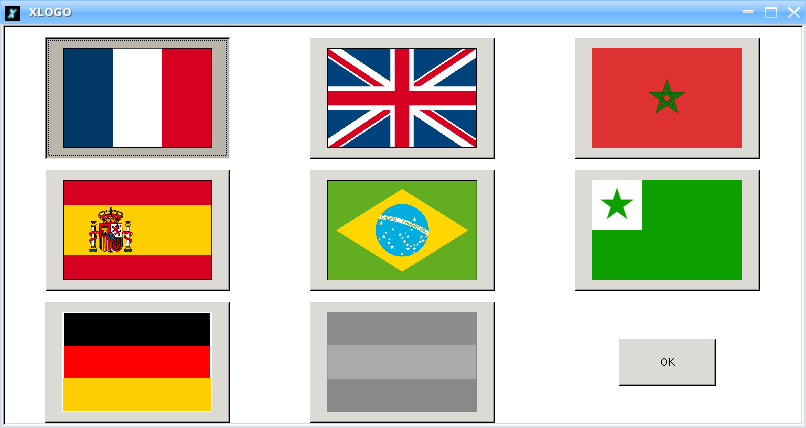
\includegraphics[scale=0.2]{bildoj/CaptureLangue.png} 
\end{center}
Tiu elekto ne estas definitiva, kompreneble; ^gin oni povas korekti
tuj per helpo de la dialogfenestro Preferoj (rigardu sekcion
\ref{onglet_general}).
\section{^Cefa fenestro}
\begin{center}
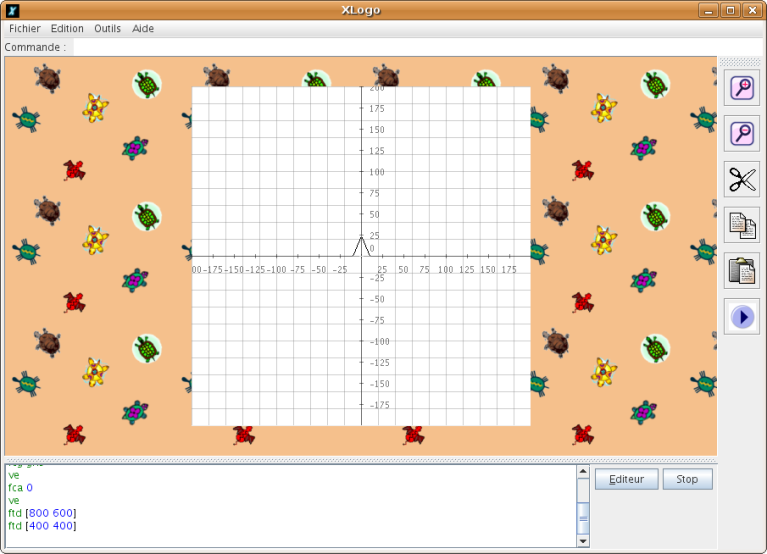
\includegraphics[scale=0.45]{bildoj/Capture.png} 
\end{center}
\begin{itemize}
\item Supre, la tradiciaj menuoj \begin{large} \textbf{Dosiero},
    \textbf{Redakti}, \textbf{Iloj} kaj \textbf{Helpo} \end{large}
\item Apude sube, \textbf{\begin{large}la komandlinio\end{large}}
  ebliganta skribi la logo-instrukciojn.
\item Meze, \begin{large}\textbf{la areo por desegni}\end{large}.
\item Dekstre de la desegnareo,
  \textbf{\begin{large}ilbreto\end{large}} vin ebligas realigi
  diversajn agojn:
\begin{itemize}
\item Zomi anta^uen/posten.
\item Diversaj redaktaj kapabloj (fortondi/kopii/alglui, tio estas,
  forigi/enpo^sigi/elpo^sigi).
\item La butono \og Legi\fg\ ebligas ruli la ^cefan komandon difinitan
  en la redaktilo.
\end{itemize}
\item Malsupre, \begin{large}\textbf{la areo \og historia
      \fg}\end{large} \ kiu memoras ^ciun lastajn komandojn tajpitajn
  kaj la respondojn rilatajn.  Por reskribi rapide instrukcion jam
  tajpitan, estas du solvoj: ^cu klaki sur la malnova instrukcio en la
  historia, ^cu klaki plurfoje sur la sago supra ^gis la instrukcio
  dezirata aperos.  La du sagoj supra kaj malsupra efektive ebligas
  movi^gi tra la tuta historio de la anta^ue tajpitaj komandoj (tre
  utile).
\item Dekstre de l' historio, du butonoj: \begin{large}\textbf{HALTI}
    kaj \textbf{REDAKTILO} \end{large}.
\begin{itemize}
\item La butono HALTI haltas ^ciun ruladon kurantan.
\item La butono REDAKTILO ebligas malfermi la proceduran redaktilon.
\end{itemize}
\end{itemize}
\section{La proceduran redaktilon}
\begin{center}
 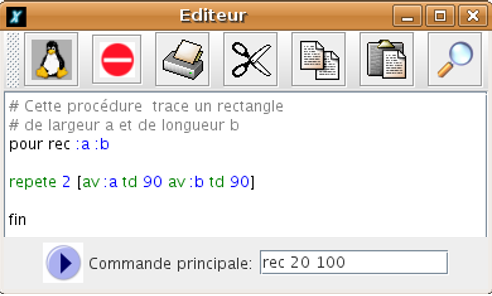
\includegraphics[scale=0.4]{bildoj/CaptureEditeur.png}
\end{center}
Por malfermi la redaktilon, tri ebloj:
\begin{itemize}
\item Tajpi \texttt{ed} en la komandlinio.  La redaktilo malfermi^gos
  tiam kun ^ciuj proceduroj jam difinitaj.  Se vi nur deziras redakti
  kelkajn procedurojn, tajpu tiam:\\
  \texttt{ed [proceduro\_1 proceduro\_2 ...]}
\item Klaku sur la butono Redaktilo de la ^cefa fenestro.
\item Uzu la klavkombinon Alt+E
\end{itemize} 
\vspace{0.5cm}
Jen la diversaj butonoj kiujn vi trovos en la redaktilo:\\

\begin{longtable}{cm{12cm}}
  \includegraphics*[scale=1]{bildoj/tortue.png} &
  Konservi la modifojn de la enhavo de la redaktilo, poste ^ci tiun
  fermi.  Ja sur tiu butono oni klaku ^ciufoje ke oni volas konservi
  la tajpitajn procedurojn.  Se vi preferas, vi povas uzi la
  klavkombinon ALT+Q. \\
  \includegraphics*[scale=1]{bildoj/quit.png} &
  Eliru la redaktilon konservante neniun modifon faritan en tiu.  Oni
  anka^u povas uzi la klavkombinon ALT+C. \\
  \includegraphics*[scale=1]{bildoj/fileprint.png} & 
  Presi la enhavon de la redaktilo.\\
  \includegraphics*[scale=1]{bildoj/editcopy.png} & 
  Kopii la elektitan tekston en la po^son.\\
  \includegraphics*[scale=1]{bildoj/editcut.png} & 
  Meti la elektitan tekston en la po^son.\\
  \includegraphics*[scale=1]{bildoj/editpaste.png} & 
  Kopii la elektitan tekston de la po^so.\\
  \includegraphics*[scale=1]{bildoj/chercher.png} &
  Malfermu dialogfenestron ebligantan ser^ci a^u anstata^uigi tekston
  en la redaktilo. \\
\end{longtable} 
\begin{center}
 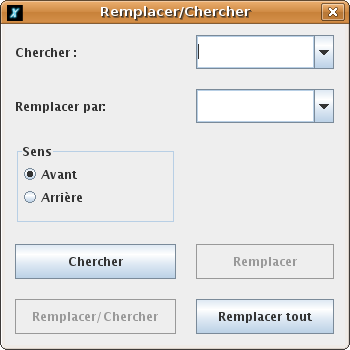
\includegraphics[scale=0.4]{bildoj/CaptureChercher.png}
\end{center}
\vspace{0.5cm}

\includegraphics{bildoj/play.png}
Malsuprege de la redaktilo, teksta kampo ebligas difini ^cefan
komandon.  ^Ci tiu reprezentas la ^generalan komandon ebligantan ruli
programon.  ^Gi estas atingebla per la butono \og legado\fg\ de la
ilbreto en la ^cefa fenestro.  Kiam oni konservas la enhavon de la
redaktilo en dosieron kun formato \texttt{.lgo}, anka^u tiu komando 
estas konservata \\ \\
\textbf{\begin{Large}GRAVE\end{Large}}: \\
\begin{itemize}
\item Neniel utilas klaki la krucon supre dekstre por fermi la
  fenestron!  Nur la du unuaj butonoj permesas eliri el la redaktilo.
\item Por forigi unu a^u plurajn procedurojn nedezirataj, uzu la
  primitivon \texttt{efp, effaceprocedure} a^u klaku en la
  menubreto \textbf{Iloj - Gestionnaire de procédures}.
\end{itemize} 
\section{Quitter}
Por eliri el XLogo, en la menubreto \textbf{Dosiero - For}, a^u klaku
la ferman krucon de la fenestro.  Dialogfenestro por konfirmi aperas
je tiu momento.
\begin{center}
 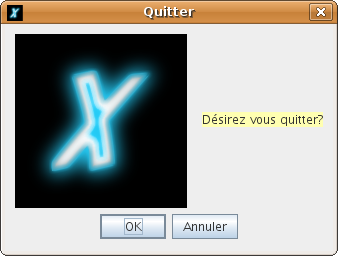
\includegraphics[scale=0.4]{bildoj/CaptureQuitter.png}
\end{center}
\chapter{Elektebloj de la menuoj:}
\section{Menu' \og Dosiero\fg}
\begin{itemize}
\item \textbf{Dosiero$\to$Nova}: detruas ^ciujn procedurojn kaj
  variabloj difinitajn por krei tiele novan laborspacon.
\item \textbf{Dosiero$\to$Malfermi}: malfermas logo-dosieron anta^ue
  konservitan.
\begin{center}
 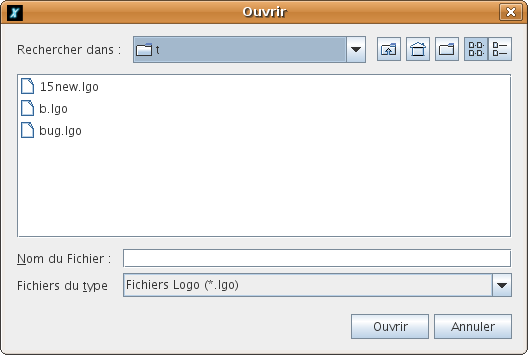
\includegraphics[scale=0.4]{bildoj/CaptureOuvrir.png}
\end{center}
\vspace{0.25cm}
\item \textbf{Dosiero$\to$Konservi kiel...}: konservas la kurantajn
  procedurojn sub elektitan nomon.
\begin{center}
 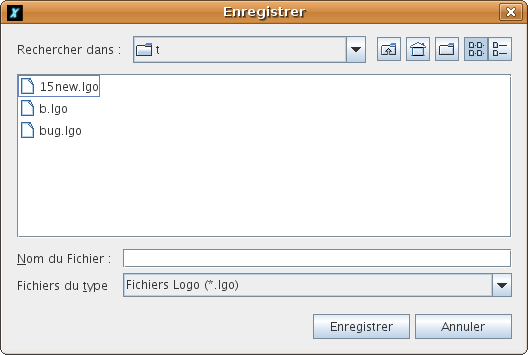
\includegraphics[scale=0.4]{bildoj/CaptureEnregistrer.png}
\end{center}
\vspace{0.25cm}
\item \textbf{Dosiero$\to$Konservi}: konservas la proceduroj en la
  dosieron nun uzatan.
\item \textbf{Dosiero$\to$Kapti la bildon$\to$Konservi la bildon
    kiel...}: ebligas konservi la bildon kun formato jpg a^u png.  Se
  vi deziras elekti nur parton de l' bildo, eblas difini elektan
  ortangulon per gliti la muson sur la desegna areo.
\item \textbf{Dosiero$\to$Kapti la bildon$\to$Presi la bildon}:
  ebligas presi la bildon.  Kiel la anta^ua, vi povas elekti ^gustan
  areon presotan.
\item \textbf{Dosiero$\to$Kapti la bildon$\to$Kopii la bildon en la
    po^son}: Ebligas sendi la bildon en la po^san sistemon.  Kiel por
  presi kaj konservi, vi povas anka^u elekti nur areon de la bildo.
  ^Gi funkcias bone en Vindozo, ne en Linukso, ne provita en
  Makinto^so.
\item \textbf{Dosiero$\to$Tekstareo$\to$Konservi je formato RTF}:
  Ebligas konservi la historian areon je formato RTF (konservas la
  kolorojn kaj formatadon de la signoj).
\item \textbf{Dosiero$\to$Eliri}: Eliri el la programo XLOGO.
\end{itemize}

\section{Menu' \og Redakti\fg}
\begin{itemize}
\item \textbf{Redakti$\to$Kopii}: Kopias la elektitan tekston en la
  po^son.
\item \textbf{Redakti$\to$Fortran^ci}: Movas la elektitan tekston en
  la po^son.
\item \textbf{Redakti$\to$Alglui}: Elpo^sigas la tekston en la
  komandlinion.
\item \textbf{Redakti$\to$Elekti ^cion}: Elektas la tutan tekston de
  la komandareo.
\end{itemize}

\section{Menu' \og Iloj\fg}
\begin{itemize}
\item \textbf{Iloj$\to$Elekti krajonan koloron}: Ebligas elekti la
  koloron per kiu skribas la testudo, helpe de koloraro.
\begin{center}
 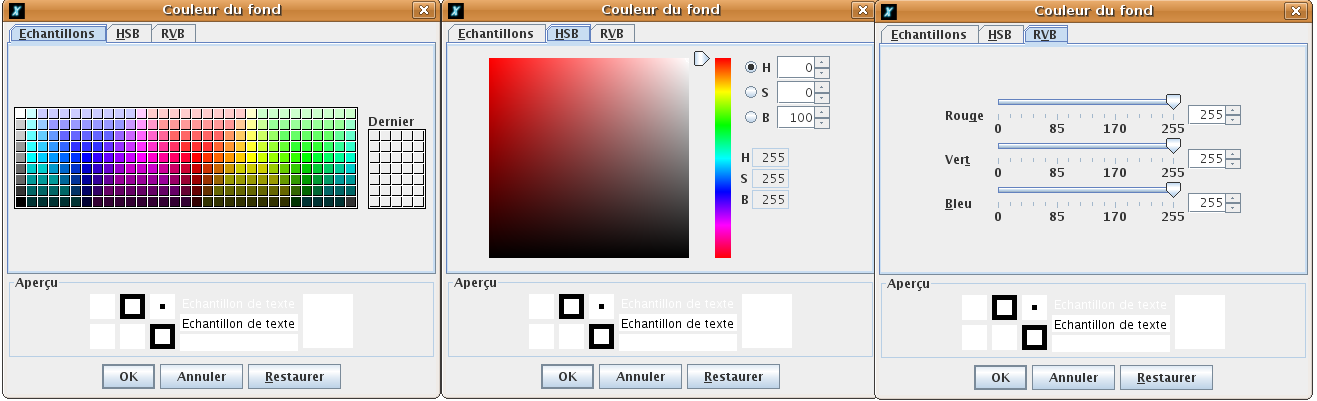
\includegraphics[scale=0.3]{bildoj/CaptureCouleur.png}
\end{center}
\vspace{0.25cm}
Havebla anka^u per la primitivo \texttt{fcc} (rigardu kroma^jon \ref{fcc}).
\item \textbf{Iloj$\to$Elekti fonkoloron}: Same pri la ekranfono.
  Havebla per la primitivo \texttt{fcfg} (rigardu kroma^jon \ref{fcfg}).
\item \textbf{Iloj$\to$Difini startodosierojn}: ebligas difini vojojn
  al dosieroj kun formato *.lgo nomataj \og startecaj\fg.  ^Ciuj
  proceduroj en tiuj dosieroj esti^gos \og kvaza^u-primitivoj\fg \ de
  la lingvo XLogo.  Ili ne estas redakteblaj nek modifeblaj de l'
  uzulo.  Vi povas anka^u difini personigitajn primitivojn.  Vi povas
  anka^u doni al ^gi komandon (en logo) rulatan dum starto de XLogo.
  Vi povas anka^u ruli programon koncipitan de vi, ekde la malfermo de
  XLogo.
  \begin{center}
    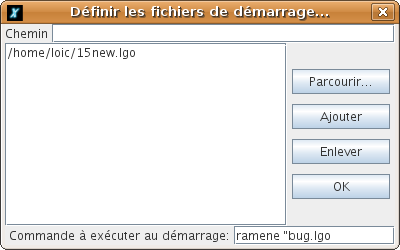
\includegraphics[scale=0.4]{bildoj/CaptureDemarrage.png}
  \end{center}
  \vspace{0.25cm}
\item \textbf{Iloj$\to$Traduki procedurojn}: Malfermas dialogfenestron
  ebligantan traduki komandojn XLogo en la lingvon deziratan.  (Tre
  utila speciale kiam oni prenas en interreto Logo-fontokodon en la
  angla, por ilin esperantigi.)
\begin{center}
 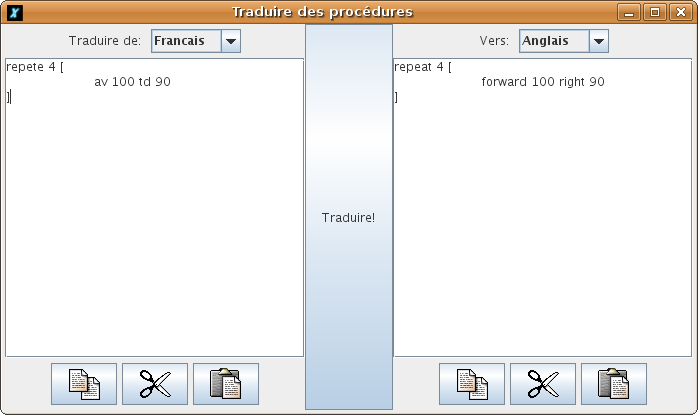
\includegraphics[scale=0.4]{bildoj/CaptureTraduire.png}
\end{center}
\vspace{0.25cm}
\item \textbf{Iloj$\to$Procedura administrilo}: Malfermas
  dialogfenestron kiu ebligas forigi procedurojn.  ^Gi permesas anka^u
  ^san^gi la aperordon de la proceduroj en la redaktilo.
\begin{center}
 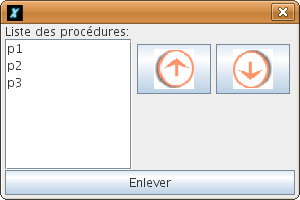
\includegraphics[scale=0.4]{bildoj/CaptureProcedure.png}
\end{center}
\vspace{0.25cm}
\item \textbf{Iloj$\to$Preferoj}: Malfermu dialogfenestron en kiu vi
  povas agordi plurajn aferojn:
  \begin{itemize} 
  \item \textbf{^Generala langeto:} \label{onglet_general}
    \begin{itemize}
    \item \textbf{Lingvo}: ^Gi ebligas elekti inter la franca, la
      angla, la hispana, la portugala, l' araba, la germana kaj
      esperanto.  Atentu, ^car la primitivoj ^san^gi^gas de lingvo al
      alia.
    \item \textbf{Aspekto:} Ebligas difini la \og look\fg on\ de la
      fenestro XLogo.  ^Cu stilo nativa, ^cu stilo Java (metala), ^cu
      stilo Motif.
    \item \textbf{Elekti la skribrapidon:} Se vi deziras vidi ^ciun
      transloki^gon de la testudo, vi povas malrapidigi ^gin helpe de
      la glitbutono celita por tio.
      \begin{center}
        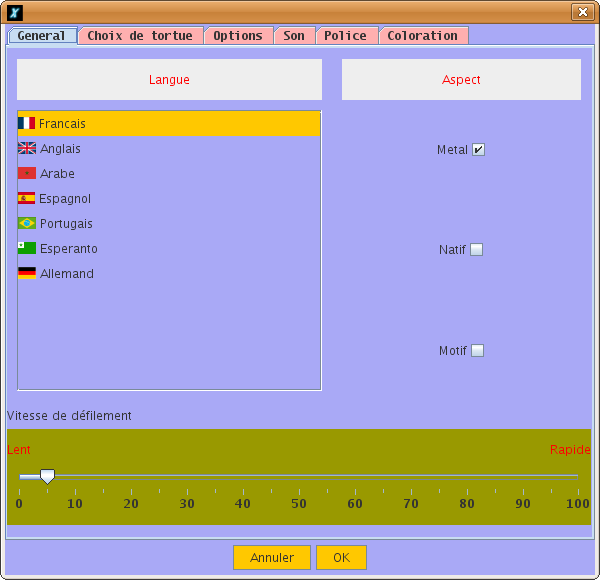
\includegraphics[scale=0.3]{bildoj/CapturePref1.png}\\
        \vspace*{1cm}
        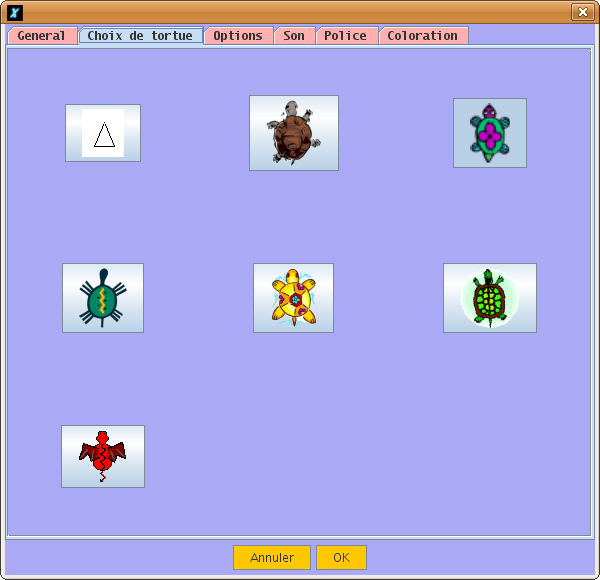
\includegraphics[scale=0.3]{bildoj/CapturePref2.png}
      \end{center}
      \vspace{0.25cm}
    \end{itemize}
  \item \textbf{Langeto Elekti testudon}: Vi povas elekti vian preferatan
    testudon.
    \begin{center}
      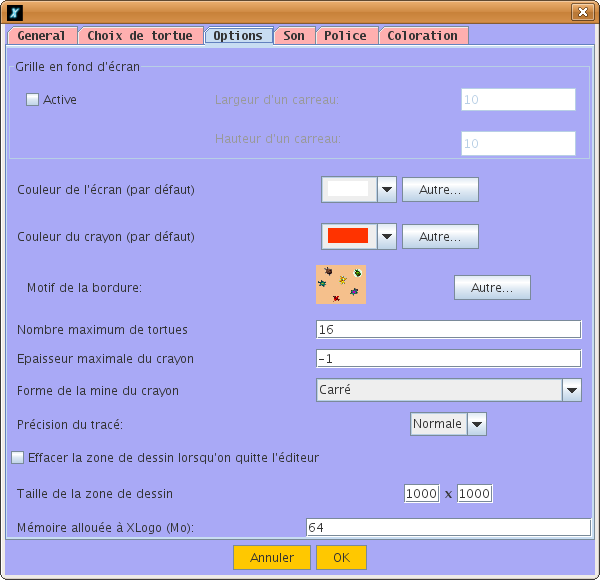
\includegraphics[scale=0.4]{bildoj/CapturePref3.png}
    \end{center}
  \item \textbf{Langeto Elektoj}: Oni povas agordi plurajn aferojn. 
    \begin{itemize}
    \item \textbf{Dratreto:} Vi povas elekti ^cu desegni dratreton sur
      l' ekranfono.  Vi povas elekti la lar^gon kaj la alton de
      kvadrato de la dratreto, kaj anka^u ^gian koloron.
    \item \textbf{Aksoj:} Vi povas elekti ^cu desegni la vertikalan
      akson kaja^u la horizontalan akson sur l' ekranfono.  Vi povas
      difini la distancon inter du gradumoj kaj anka^u la koloron de
      ^ciu akso.
    \item \textbf{Koloro de ekranfono}: Eblo difini aprioran koloron
      de ekranfono.
    \item \textbf{Koloro de krajono}: Eblo difini aprioran koloron
      krajonan.
    \item \textbf{Bordera motivo}: Eblo difini preciza motivon por la
      mar^geno enkadriganta la desegnejon (^cu per bildo, ^cu per nura
      koloro)
      \begin{center}
        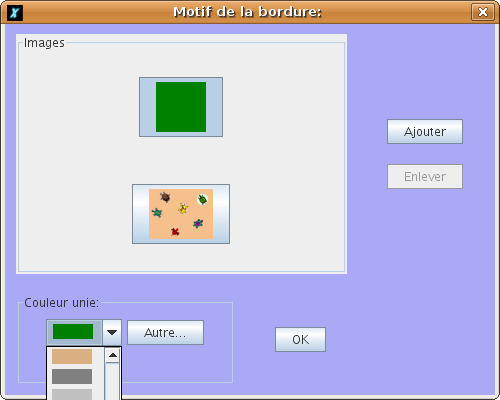
\includegraphics[scale=0.4]{bildoj/CaptureBordure.png}
      \end{center}
    \item \textbf{Diko de krajono}: Oni povas indiki liman amplekson
      por la dikeco de krajono.  Si oni ne volas uzi tiun limigon,
      metu la nombron $-1$ en la areon tekstan rilatan.
    \item \textbf{Formo de krajono}: Tuj, oni povas elekti la formon
      de la testuda krajono.  Por ^gin rimarki, elektu krajondikon pli
      grandan ol $1$.
    \item \textbf{Maksimuma nombro de testudoj}: Oni povas ^san^gi la
      maksimuman nombron de testudoj en plurtestuda moduso (apriore
      16).
    \item \textbf{Desegna precizeco}: Vi povas elekti la desegnan
      kvaliton.  Je alta kvalito, vi ne havos la efikon de
      linipikselado.  Male, atentu ke, ju pli da kvalito, des malpli da
      rulrapideco.
    \item \textbf{Purigado je eliro el redaktilo}: Oni povas elekti
      ^cu a^utomate purigi la desegnejon kiam oni eliras el la
      redaktilo.
    \item \textbf{Amplekso de la desegnejo}: Vi povas elekti propran
      amplekson por la desegnejo.  Apriore XLogo ruli^gas kun areo de
      1000 pikseloj mul 1000 pikseloj. \textcolor{red} {Atentu:} Kiam
      vi pligrandigas la bildon, eble necesas pligrandigi la kvanton
      de memoro atribuita al XLogo.  Erarmesa^go vin avertos pri tio.
    \item \textbf{Memoro atribuita al XLogo}: Vi povas tial anka^u
      ^san^gi la valoron rilatan al la memora spaco atribuita al
      XLogo.  Apriore, tiu valoro estas 64 MiB.  Eble vi devos
      pligrandigi ^gin se vi deziros labori sur desegnejo pli granda.
      Kiam oni modifas tiun parametron, la ^san^go nur efikas post la
      restarto de XLogo. \textcolor{red} {Atentu, ne pligrandigu multe
        sen ka^uzo tiun valoron; ^gi povas multe malrapidigi vian
        sistemon.}
    \item \textbf{Nombro de pordo TCP:} Ebligas elekti iun valoron por
      la pordo uzata por la retkomunikadoj.  Rigardu
      p.~\pageref{reseau}.
    \end{itemize}
    \begin{center}
      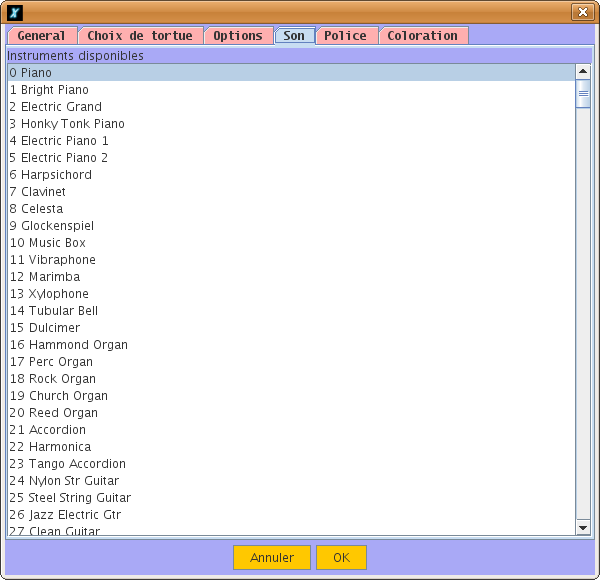
\includegraphics[scale=0.4]{bildoj/CapturePref4.png}
    \end{center}
    \vspace{0.25cm}
  \item \textbf{Langeto Sono}: vi trovos la liston de instrumentoj
    kiujn povas ^sajnigi via sonkarto per l' interfaco MIDI.  Vi povas
    elekti instrumenton klakante ^gian nomon.  (Vi povas elekti
    instrumenton anka^u per la primitivo \texttt{instrumenton\_provizu
      numero}.)  Se la listo de instrumentoj ne aperas, rigardu la
    Oftajn Demandojn fine de l' gvidlibro pri tiu afero.
    \begin{center}
      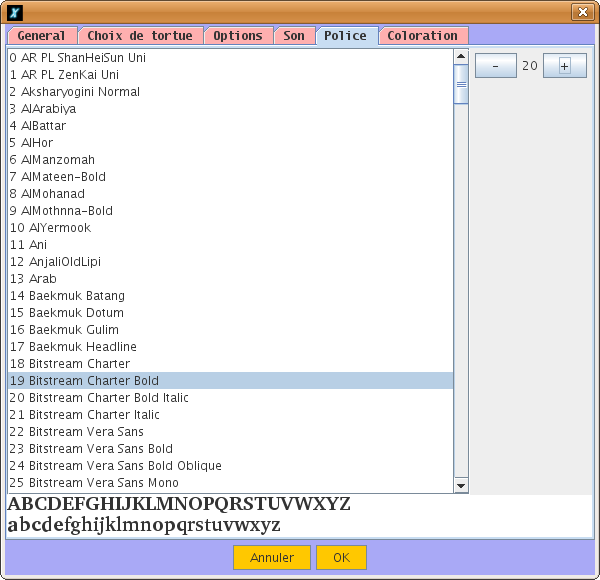
\includegraphics[scale=0.4]{bildoj/CapturePref5.png}
    \end{center}
    \vspace{0.25cm}
  \item \textbf{Langeto Tiparo}: En la kvina langeto, vi povas elekti
    la tiparon de la grafika interfaco kaj ^gian amplekson.  Atentu ke
    tio ne influas la tiparon uzatan de la primitivoj \texttt{skribu}
    et \texttt{etikedu}.
    \begin{center}
      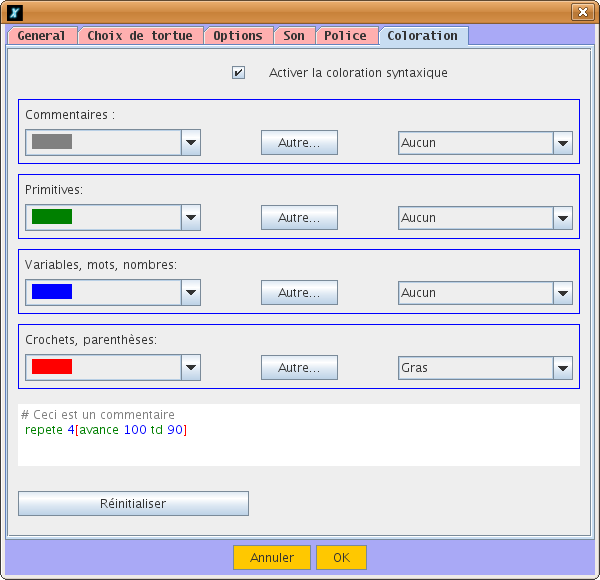
\includegraphics[scale=0.4]{bildoj/CapturePref6.png}
    \end{center}
    \vspace{0.25cm}
  \item \textbf{Langeto Sintaksa kolorigo}: Eblo (mal)aktivigi la
    sintaksan kolorigon kaj difini proprajn kolorojn.
\end{itemize}
\end{itemize}
\section{Menu' \og Helpo\fg}
\begin{itemize}
\item \textbf{Menu' Helpo$\to$Reta lernolibro}: Aliras la referencan
  lernolibron de \xlogo, nur se ekzistas interreta konekto.
  \vspace{0.25cm}
\item \textbf{Menu' Helpo$\to$Permesilo}: Aliras la permesilon GPL sub
  kiu oni distribuas la programon.
  \begin{center}
    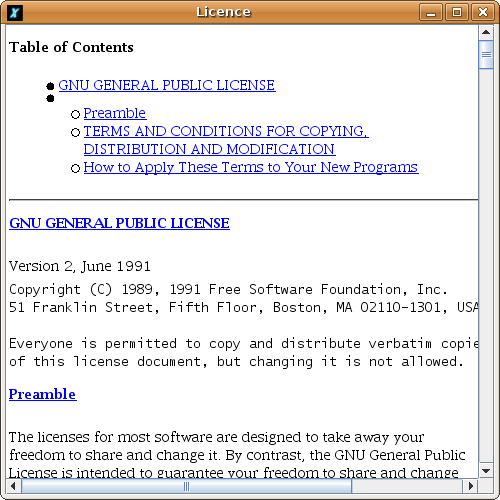
\includegraphics[scale=0.4]{bildoj/CaptureLicence.png}
  \end{center}
  \vspace{0.25cm}
\item \textbf{Menu' Helpo$\to$Esperanta traduko}: Aliras
  esperantigitan permesilon GPL.  Tiu traduka^jo havas nenian valoron
  oficialan, nur la angla originalo.

\item \textbf{Menu' Helpo$\to$Traduki XLogo-n}: Malfermas
  dialogfenestron ebligantan konsulti / modifi / kompletigi la aron de
  traduka^joj de XLogo (mesa^goj kaj primitivoj).
  \begin{center}
    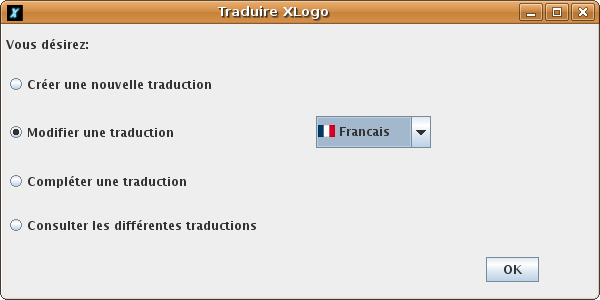
\includegraphics[scale=0.4]{bildoj/CaptureXLogoTrad1.png}
    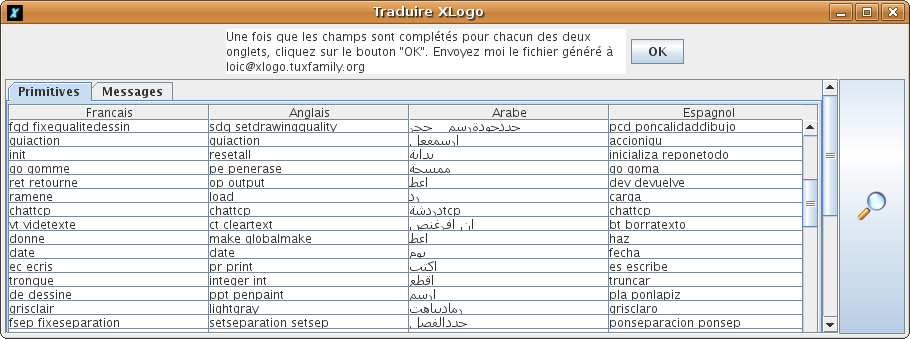
\includegraphics[scale=0.4]{bildoj/CaptureXLogoTrad2.png}
  \end{center}
  \vspace{0.25cm} Eblas anka^u krei traduka^jojn por nova
  lingvo.  Je ^ciu okazo oni sendu la dosieron generitan al
  \url{loic@xlogo.tuxfamily.org}.
\item \textbf{Menu' Helpo$\to$Rilate...}: Klasika ... kaj
  \url{http://xlogo.tuxfamily.org} por viaj ^gisdatigoj!!
  \texttt{o:)}
  \begin{center}
    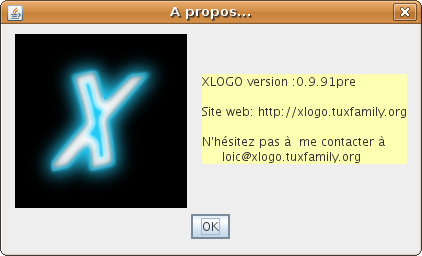
\includegraphics[scale=0.6]{bildoj/CaptureApropos.png}
  \end{center}
  \vspace{0.25cm}
\end{itemize}


